\section{Multicore Architectures}

\subsection{Explore the CPU}

\begin{lstlisting}[caption=Output from lscpu command]
-bash-4.1$ lscpu
Architecture:          x86_64
CPU op-mode(s):        32-bit, 64-bit
Byte Order:            Little Endian
CPU(s):                32
On-line CPU(s) list:   0-31
Thread(s) per core:    2
Core(s) per socket:    8
Socket(s):             2
NUMA node(s):          4
Vendor ID:             AuthenticAMD
CPU family:            21
Model:                 1
Model name:            AMD Opteron(TM) Processor 6274
Stepping:              2
CPU MHz:               1400.000
BogoMIPS:              4399.38
Virtualization:        AMD-V
L1d cache:             16K
L1i cache:             64K
L2 cache:              2048K
L3 cache:              6144K
NUMA node0 CPU(s):     0-7
NUMA node1 CPU(s):     8-15
NUMA node2 CPU(s):     16-23
NUMA node3 CPU(s):     24-31
\end{lstlisting}

We see that 32 logical CPU cores and this is shared across 2 physical CPUs with
8 cores each which are dual threaded. Resulting in $2 \times 8 \times 2 = 32$.

\begin{figure}
    \centering
    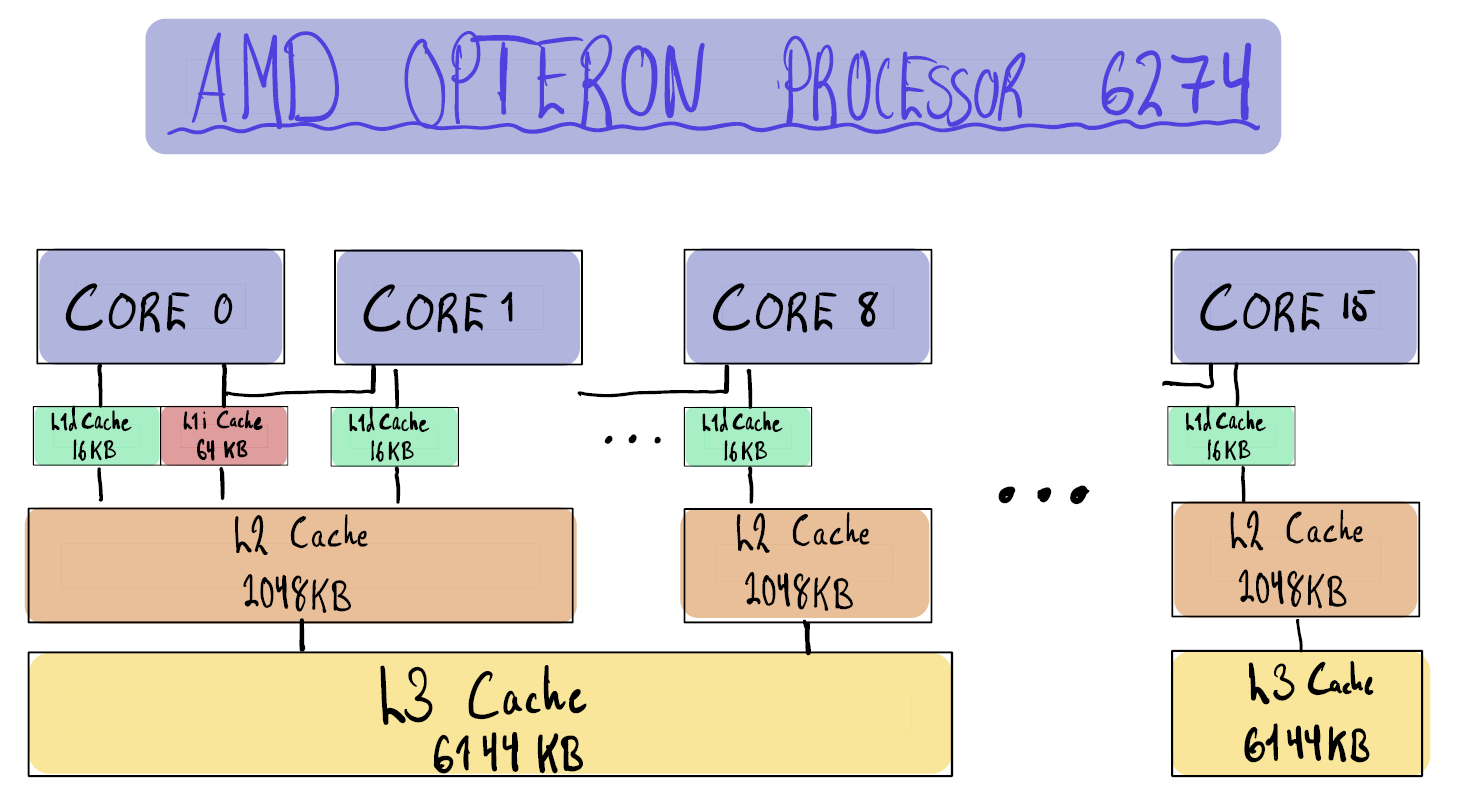
\includegraphics[width=\linewidth]{Figures/datahierarchy.PNG}
    \caption{Cache Hierarchy of AMD Opteron Processor 6274 om gullviva.it.uu.se}
\end{figure}

We see that this processor has a lot more physical cores. In summary we have:

\begin{itemize}
    \item There are in total 2 physical CPUs. Each with 8 physical cores.
    \item Each physical core has two logical CPUs.
    \item Each physical core has an L1d, L1i and L2 cache of sizes 16, 64, AND 2048KB respectively.
    \item Four physical cores share one L3 cache of size 6144KB.
\end{itemize}

We see that the caches are somewhat similar. The L2 cache fo each physical core
have more memory compared to the Intel I5-450M processors. The L3 cache is also 
larger but share 4 physical cores instead of 2. The main difference is that 
there are a lot more physical and logical cores, which will allow for concurrent
multithreaded programming.